% https://www.overleaf.com/project/new/template/19345?id=65231945&templateName=An+example+of+the+beamer+package&latexEngine=&texImage=texlive-full%3A2020.1&mainFile=
% https://www.overleaf.com/learn/latex/Beamer#Further_reading
\PassOptionsToPackage{dvipsnames}{xcolor}
\documentclass{beamer}
\addtobeamertemplate{navigation symbols}{}{%
    \usebeamerfont{footline}%
    % \setbeamerfont{footline}{series=\bfseries}
    % \usebeamercolor[fg]{footline}%
    % \setbeamercolor{footline}{fg=blue}
    \hspace{1em}%
    \raisebox{1.3pt}{\insertframenumber/\inserttotalframenumber}
}
\usepackage[UTF8]{ctex}
\setCJKsansfont[BoldFont=NotoSansSC-Bold.otf]{NotoSansSC-Regular.otf}
\usepackage{outlines}
\usepackage{subfigure}
\usepackage{bbm}
\usepackage[outputdir=../]{minted}
% \usepackage[utf8]{inputenc}
% \usepackage{CJKutf8}
\usetheme{Berkeley}
\usecolortheme{seahorse}
\colorlet{SlightGray}{Gray!8}

%------------------------------------------------------------
%This block of code defines the information to appear in the
%Title page
\title[SE x AI] %optional
{深度学习编译器模糊测试工具的拓展}

\subtitle{中期报告}

\author[] % (optional)
{彭晋钧\inst{1}}

\institute[VFU] % (optional)
{
  \inst{1}%
  计算机科学与技术系\\
  清华大学\\
  \vspace{1em}
  指导教师:韩文弢\\
  校外指导:Lingming Zhang (UIUC)
}

\date[2023] % (optional)
{本科生综合论文训练, 2023}

%End of title page configuration block
%------------------------------------------------------------

%------------------------------------------------------------
%The next block of commands puts the table of contents at the 
%beginning of each section and highlights the current section:

\AtBeginSection[]
{
  \begin{frame}
    \frametitle{Table of Contents}
    \tableofcontents[currentsection]
  \end{frame}
}
%------------------------------------------------------------

\begin{document}
% \begin{CJK}{UTF8}{gbsn}

%The next statement creates the title page.
\frame{\titlepage}

%---------------------------------------------------------
%This block of code is for the table of contents after
%the title page
\begin{frame}
\frametitle{Table of Contents}
\tableofcontents
\end{frame}
%---------------------------------------------------------

\section{Background}

\subsection{Deep Learning Compilers}
\begin{frame}{Background - Deep Learning Compilers}
    Neural Networks
    \begin{itemize}
        \item computational graph
        \item DAG
    \end{itemize}
    Deep Learning Compilers
    \begin{itemize}
        \item Optimize computational graphs representing neural networks
        \item Constant folding, Operator fusion, ...
        \item XLA for TensorFlow, PyTorch JIT, TorchDynamo and TorchInductor
    \end{itemize}
\end{frame}

\subsection{Fuzzing}
\begin{frame}{Background - Fuzzing}
    \begin{itemize}
        \item Feed random inputs into program to test\\
        e.g. Input random strings to Unix programs
        \item Unexpected behavior $\rightarrow$ Bug!
        \item Input for deep learning compilers: NN/computational graph
        \item more diverse input graph $\rightarrow$ higher coverage \& more potential bugs
    \end{itemize}
\end{frame}


\section{Related Works}
\subsection{Related Works - API-level Fuzzing}
\begin{frame}{Related Works - API-level Fuzzing}
    API-level Fuzzing: FreeFuzz (ICSE'22)
    \begin{itemize}
        \item \texttt{torch.add(x, y)}
        \item "free": collect traces from unit tests and public repos
        \item limitation: cannot test graph optimizations in compilers
    \end{itemize}
\end{frame}

\subsection{Related Works - Graph-level Fuzzing}
\begin{frame}{Related Works - Graph-level Fuzzing}
    Graph-level Fuzzing: how to match tensor shapes between operators?
    \begin{itemize}
        \item LEMON, Muffin: preserve tensor shapes
        \begin{itemize}
            \item shape-preserving operators (e.g. \texttt{relu})
            \item append additional operators (e.g. \texttt{Linear, reshape})
            \item limitation: not real world usages
        \end{itemize}
        \item NNSmith (ASPLOS'22)
        \begin{itemize}
            \item symbolically define a set of operators
            \begin{itemize}
                \item $\text{output shapes = f(\text{input shapes})}$
                \item constraints on input shapes
            \end{itemize}
            \item symbolically generate a \textit{valid} graph/DNN
            \item limitation: involves lots of human effort to write symbolic rules
        \end{itemize}
    \end{itemize}
\end{frame}

\section{Main Work}

\subsection{Overview}
\begin{frame}{Overview}
    \begin{figure}
        \centering
        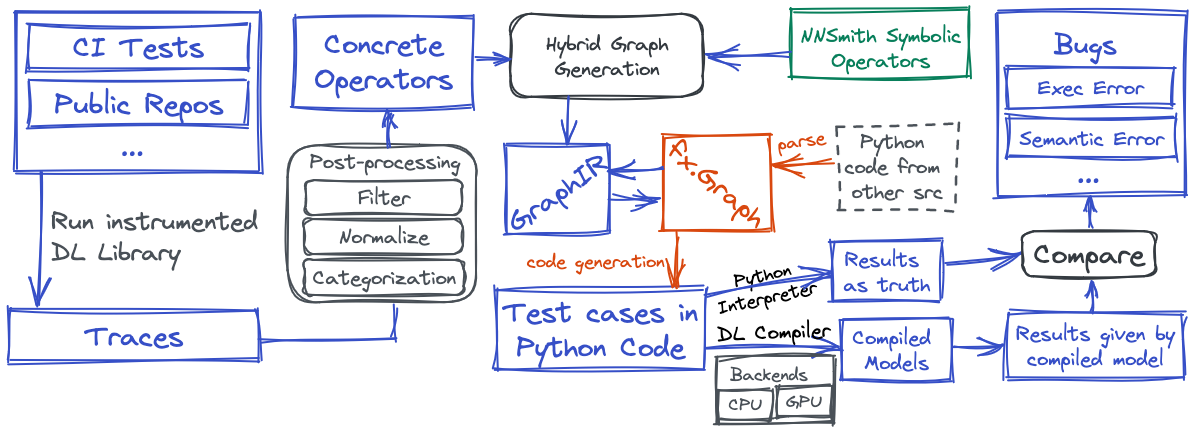
\includegraphics[scale=0.225]{figs/overview.png}
        \label{fig:overview}
    \end{figure}
\end{frame}

\subsection{Hybrid Graph Generation}
\begin{frame}{Hybrid Graph Generation}
    Traces collection by instrumentation
    \begin{itemize}
        \item real world usages of APIs
        \item similar to FreeFuzz
    \end{itemize}
    Previous symbolic generation:
    \begin{itemize}
        \item symbolic operators $\rightarrow$ whole symbolic graph $\rightarrow$ invoke SMT solver to get a concrete graph
    \end{itemize}
    Hybrid generation
    \begin{itemize}
        \item At each step, insert a symbolic operator or a concrete operator.
        \item Concretize the graph immediately at each step.
    \end{itemize}
\end{frame}

\begin{frame}{Hybrid Graph Generation}
    Evaluation on PyTorch (branch coverage)
    \begin{itemize}
        \item NNSmith: 40.0k / 258k
        \item Ours: 45.5k / 258k ; 13.8\% improvement
    \end{itemize}
    Bug sample:
    \begin{figure}
        \centering
        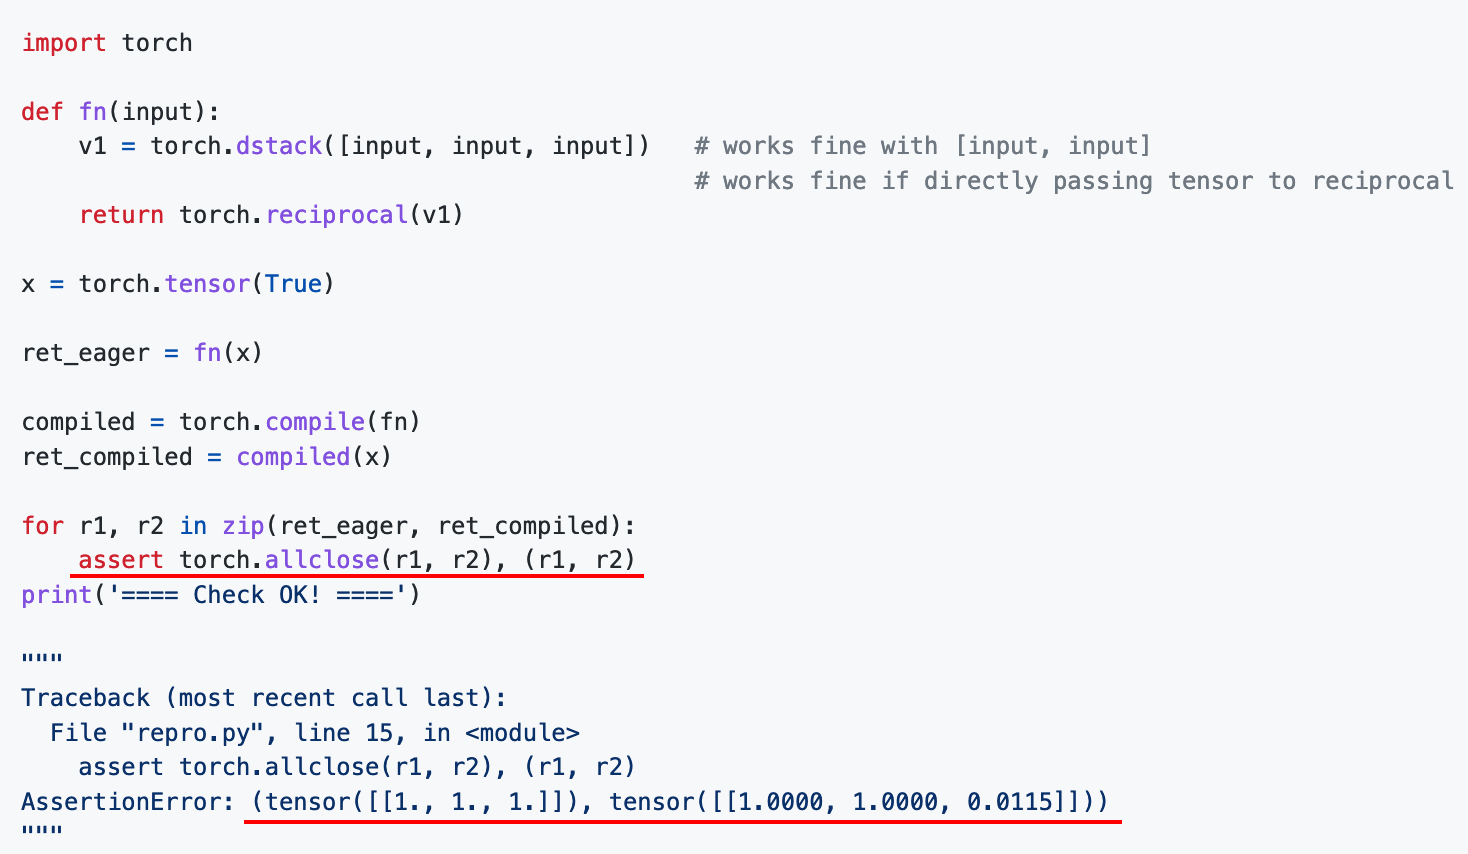
\includegraphics[scale=0.18]{figs/bug_sample.png}
        \label{fig:bug_sample}
    \end{figure}
\end{frame}

\subsection{Code Generation}
\begin{frame}{Code Generation}
    NNSmith: do forward propagation in a complex for-loop
    \begin{itemize}
        \item a container for all intermediate variables
        \item a container for all operators (callable functions and \texttt{nn.Module})
    \end{itemize}
    Issues of NNSmith bug reports:
    \begin{itemize}
        \item not similar to real-world human written models
        \item compilers may break the graph into several components $\rightarrow$ lose possible graph-level optimizations
        \item very hard to debug/minimize; time-consuming
    \end{itemize}
    Ours: generate clean \& simple codes for forward propagation
    \begin{itemize}
        \item generate graphs as GraphIR
        \item generate (Python) codes based on GraphIR
    \end{itemize}
\end{frame}

\begin{frame}[fragile]{Code Generation}
    Sample of generated code:
    % \begin{columns}
    %     \column{0.5\textwidth}
    %     \begin{figure}
    %         \centering
    %         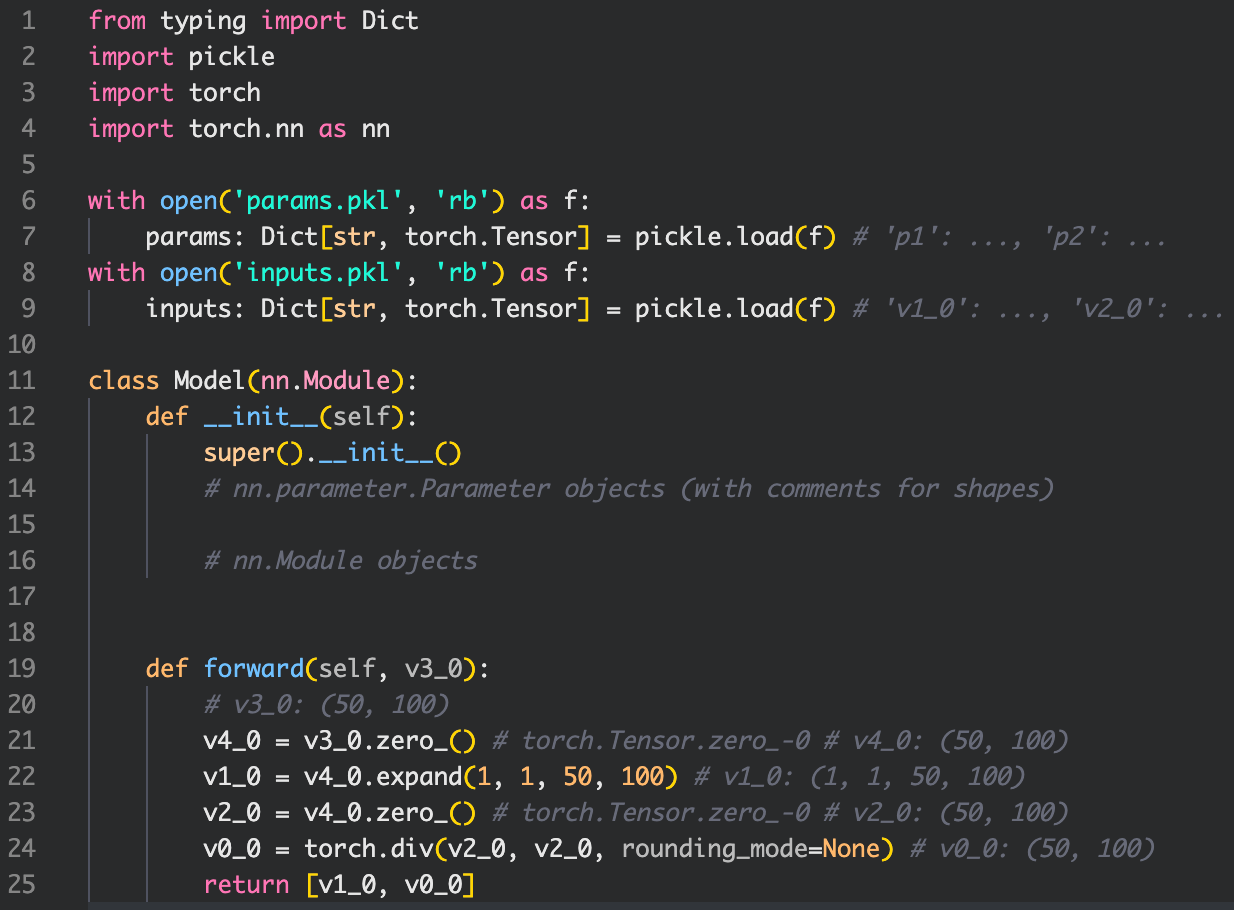
\includegraphics[scale=0.125]{figs/gen_code_0.png}
    %         \label{fig:gen_code_0}
    %     \end{figure}
    %     \column{0.5\textwidth}
    %     \begin{figure}
    %         \centering
    %         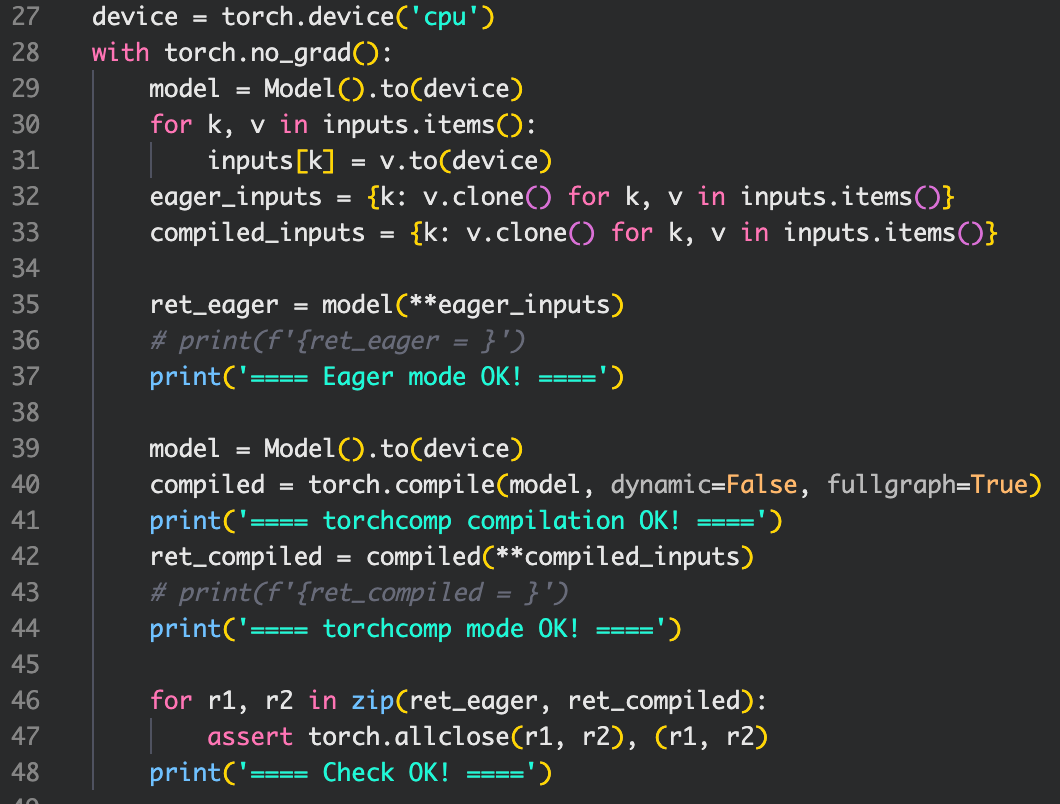
\includegraphics[scale=0.13]{figs/gen_code_1.png}
    %         \label{fig:gen_code_1}
    %     \end{figure}
    % \end{columns}
    \begin{columns}
    \column{0.02\textwidth}
    \column{0.98\textwidth}
        \begin{minted}[
            fontsize=\tiny,
            linenos,
            frame=lines,
            framesep=1.5mm,
            bgcolor=SlightGray,
        ]{python}
from typing import Dict
import pickle
import torch
import torch.nn as nn

with open('params.pkl', 'rb') as f:
    params: Dict[str, torch.Tensor] = pickle.load(f) # 'p1': ..., 'p2': ...
with open('inputs.pkl', 'rb') as f:
    inputs: Dict[str, torch.Tensor] = pickle.load(f) # 'v1_0': ..., 'v2_0': ...

class Model(nn.Module):
    def __init__(self):
        super().__init__()
        # nn.parameter.Parameter objects (with comments for shapes)

        # nn.Module objects


    def forward(self, v3_0):
        # v3_0: (50, 100)
        v4_0 = v3_0.zero_() # torch.Tensor.zero_-0 # v4_0: (50, 100)
        v1_0 = v4_0.expand(1, 1, 50, 100) # v1_0: (1, 1, 50, 100)
        v2_0 = v4_0.zero_() # torch.Tensor.zero_-0 # v2_0: (50, 100)
        v0_0 = torch.div(v2_0, v2_0, rounding_mode=None) # v0_0: (50, 100)
        return [v1_0, v0_0]
    \end{minted}
    \end{columns}
\end{frame}

\subsection{Extension for AI-assisted Model Generation}
\begin{frame}{Extension for AI-assisted Model Generation}
    Utilize previous bug reports or ChatGPT
    \begin{itemize}
        \item Parse existing model definitions to GraphIR
        \item Do mutation to generate new cases ("locality")
    \end{itemize}
    Parsing
    \begin{itemize}
        \item PyTorch tracing/TorchDynamo:\\Python code $\rightarrow$ PyTorch IR
        \item Our converter: PyTorch IR $\rightarrow$ our GraphIR
    \end{itemize}
\end{frame}

\subsection{Empirical Study on Root Causes}
\begin{frame}{Empirical Study on Root Causes}
    \begin{itemize}
        \item Track progress of submitted issues
        \item Analyze developers' commit records and discussions to learn root causes
        \item Inspire future research: efficient debugging
    \end{itemize}
\end{frame}

\begin{frame}{The End}
    Thank you!    
\end{frame}

% \end{CJK}
\end{document}



\iffalse

%------------------------------------------------------------
%This block of code defines the information to appear in the
%Title page
\title[About Beamer] %optional
{About the Beamer class in presentation making}

\subtitle{A short story}

\author[Arthur, Doe] % (optional)
{A.~B.~Arthur\inst{1} \and J.~Doe\inst{2}}

\institute[VFU] % (optional)
{
  \inst{1}%
  Faculty of Physics\\
  Very Famous University
  \and
  \inst{2}%
  Faculty of Chemistry\\
  Very Famous University
}

\date[VLC 2021] % (optional)
{Very Large Conference, April 2021}

\logo{\includegraphics[height=1cm]{overleaf-logo}}

%End of title page configuration block
%------------------------------------------------------------

%------------------------------------------------------------
%The next block of commands puts the table of contents at the 
%beginning of each section and highlights the current section:

\AtBeginSection[]
{
  \begin{frame}
    \frametitle{Table of Contents}
    \tableofcontents[currentsection]
  \end{frame}
}
%------------------------------------------------------------


\begin{document}
\begin{CJK}{UTF8}{gbsn}

%The next statement creates the title page.
\frame{\titlepage}


%---------------------------------------------------------
%This block of code is for the table of contents after
%the title page
\begin{frame}
\frametitle{Table of Contents}
\tableofcontents
\end{frame}
%---------------------------------------------------------


\section{First section}

\subsection{Item}

\subsubsection{What?}

%---------------------------------------------------------
%Changing visivility of the text
\begin{frame}
\frametitle{Show item}
This is a text in second frame. For the sake of showing an example.

\begin{itemize}
    \item<1-> Text visible on slide 1
    \item<2-> Text visible on slide 2
    \item<3> Text visible on slides 3
    \item<4-> Text visible on slide 4
\end{itemize}
\end{frame}

%---------------------------------------------------------

\subsection{Pause}

%---------------------------------------------------------
%Example of the \pause command
\begin{frame}
\frametitle{Show pause}
In this slide \pause

the text will be partially visible \pause

And finally everything will be there
\end{frame}
%---------------------------------------------------------

\subsection{Pause2}

%---------------------------------------------------------
%Example of the \pause command
\begin{frame}
\frametitle{Show pause 2}
In this slide \pause

the text will be partially visible \pause

And finally everything will be there
\end{frame}
%---------------------------------------------------------

\subsection{Pause3}

%---------------------------------------------------------
%Example of the \pause command
\begin{frame}
\frametitle{Show pause 3}
In this slide \pause

the text will be partially visible \pause

And finally everything will be there
\end{frame}
%---------------------------------------------------------

\section{Second section}

%---------------------------------------------------------
%Highlighting text
\begin{frame}
\frametitle{Sample frame title}

In this slide, some important text will be
\alert{highlighted} because it's important.
Please, don't abuse it.

\begin{block}{Remark}
Sample text
\end{block}

\begin{alertblock}{Important theorem}
Sample text in red box
\end{alertblock}

\begin{examples}
Sample text in green box. The title of the block is ``Examples".
\end{examples}
\end{frame}
%---------------------------------------------------------


%---------------------------------------------------------
%Two columns
\begin{frame}
\frametitle{Two-column slide}

\begin{columns}

\column{0.5\textwidth}
This is a text in first column.
$$E=mc^2$$
\begin{itemize}
\item First item
\item Second item
\end{itemize}

\column{0.5\textwidth}
This text will be in the second column
and on a second tought this is a nice looking
layout in some cases.
\end{columns}
\end{frame}
%---------------------------------------------------------

\end{CJK}
\end{document}

\fi
